\section{Attach Handles}

Stratifying $M$ allows the definition of attachment neighbourhoods for stratified 2--, 3--, and 4--handles in $W=M\times\Ilit$.
A 4--dimensional 2--handle is attached over a closed solid torus embedded in the boundary of a 4--manifold, so attachment neighbourhoods for our stratified 2--handles are straightforward: they are the face blocks of $M$.
We alter the boundary of $W$ by attaching handles, so the attachment neighbourhoods for 3--handles (4--handles, resp.) must be found after 2--handles (3--handles, resp.) are attached.
For a 3--handle, an attachment neighbourhood consists of the union of an edge block with some strata introduced by 2--handle attachment.
For a 4--handles, an attachment neighbourhood consists of the union of an edge block with some strata introduced by 2-- and 3--handle attachment.
We investigate the consequences of handle attachment by comparing the boundary of the initial manifold with the boundary of the manifold resulting from handle attachment, and use a precisely defined handle structure to focus the investigation.
Our first step is to precisely define the structure of the stratified 2--handles that we are attaching.

\subsection{2--handles}

Let $B$ be a face block of $M_1$.
By Theorem \ref{thm:block-structure}, $B$ is a closed solid torus that is stratified-homeomorphic to $S^1\times G_n$, where $G_n$ is an $n$--gon for some $n$.
Consider an unknotted embedding of $B$ in $S^3$.
The complement of the interior of $B$ is another closed solid torus $B'$.
The tori $B$ and $B'$ are depicted as cylinders with top and bottom identified in Figure \ref{fig:face-block-complement}.

We stratify $B'$ as follows.
First include the shared stratified boundary of $B$.
Next, introduce meridinal disks of $B'$ that are bounded by the $(1,i)$--indexed strata in $B$, i.e.\ the boundary curves in $B$ corresponding to $S^1\times c_m$ where $c_m$ is a corner of $G_n$, $m=1\dots n$.
Finally, add the homeomorphic 3--disks of $B'$ whose boundaries consist of one longitudinal annulus of $B$ along with the two meridinal disks in $B'$ that are bounded by the annulus's circular boundary components.
The filtration of $B'$ is created identically to that of the original face blocks, using inclusion as a partial ordering and indexing a stratum by its dimension as a submanifold of $B'$.
Figure \ref{fig:face-block-complement} illustrates a face block $B$ and its complement inside of $S^3$.

\begin{figure}[h!]
	\centering
	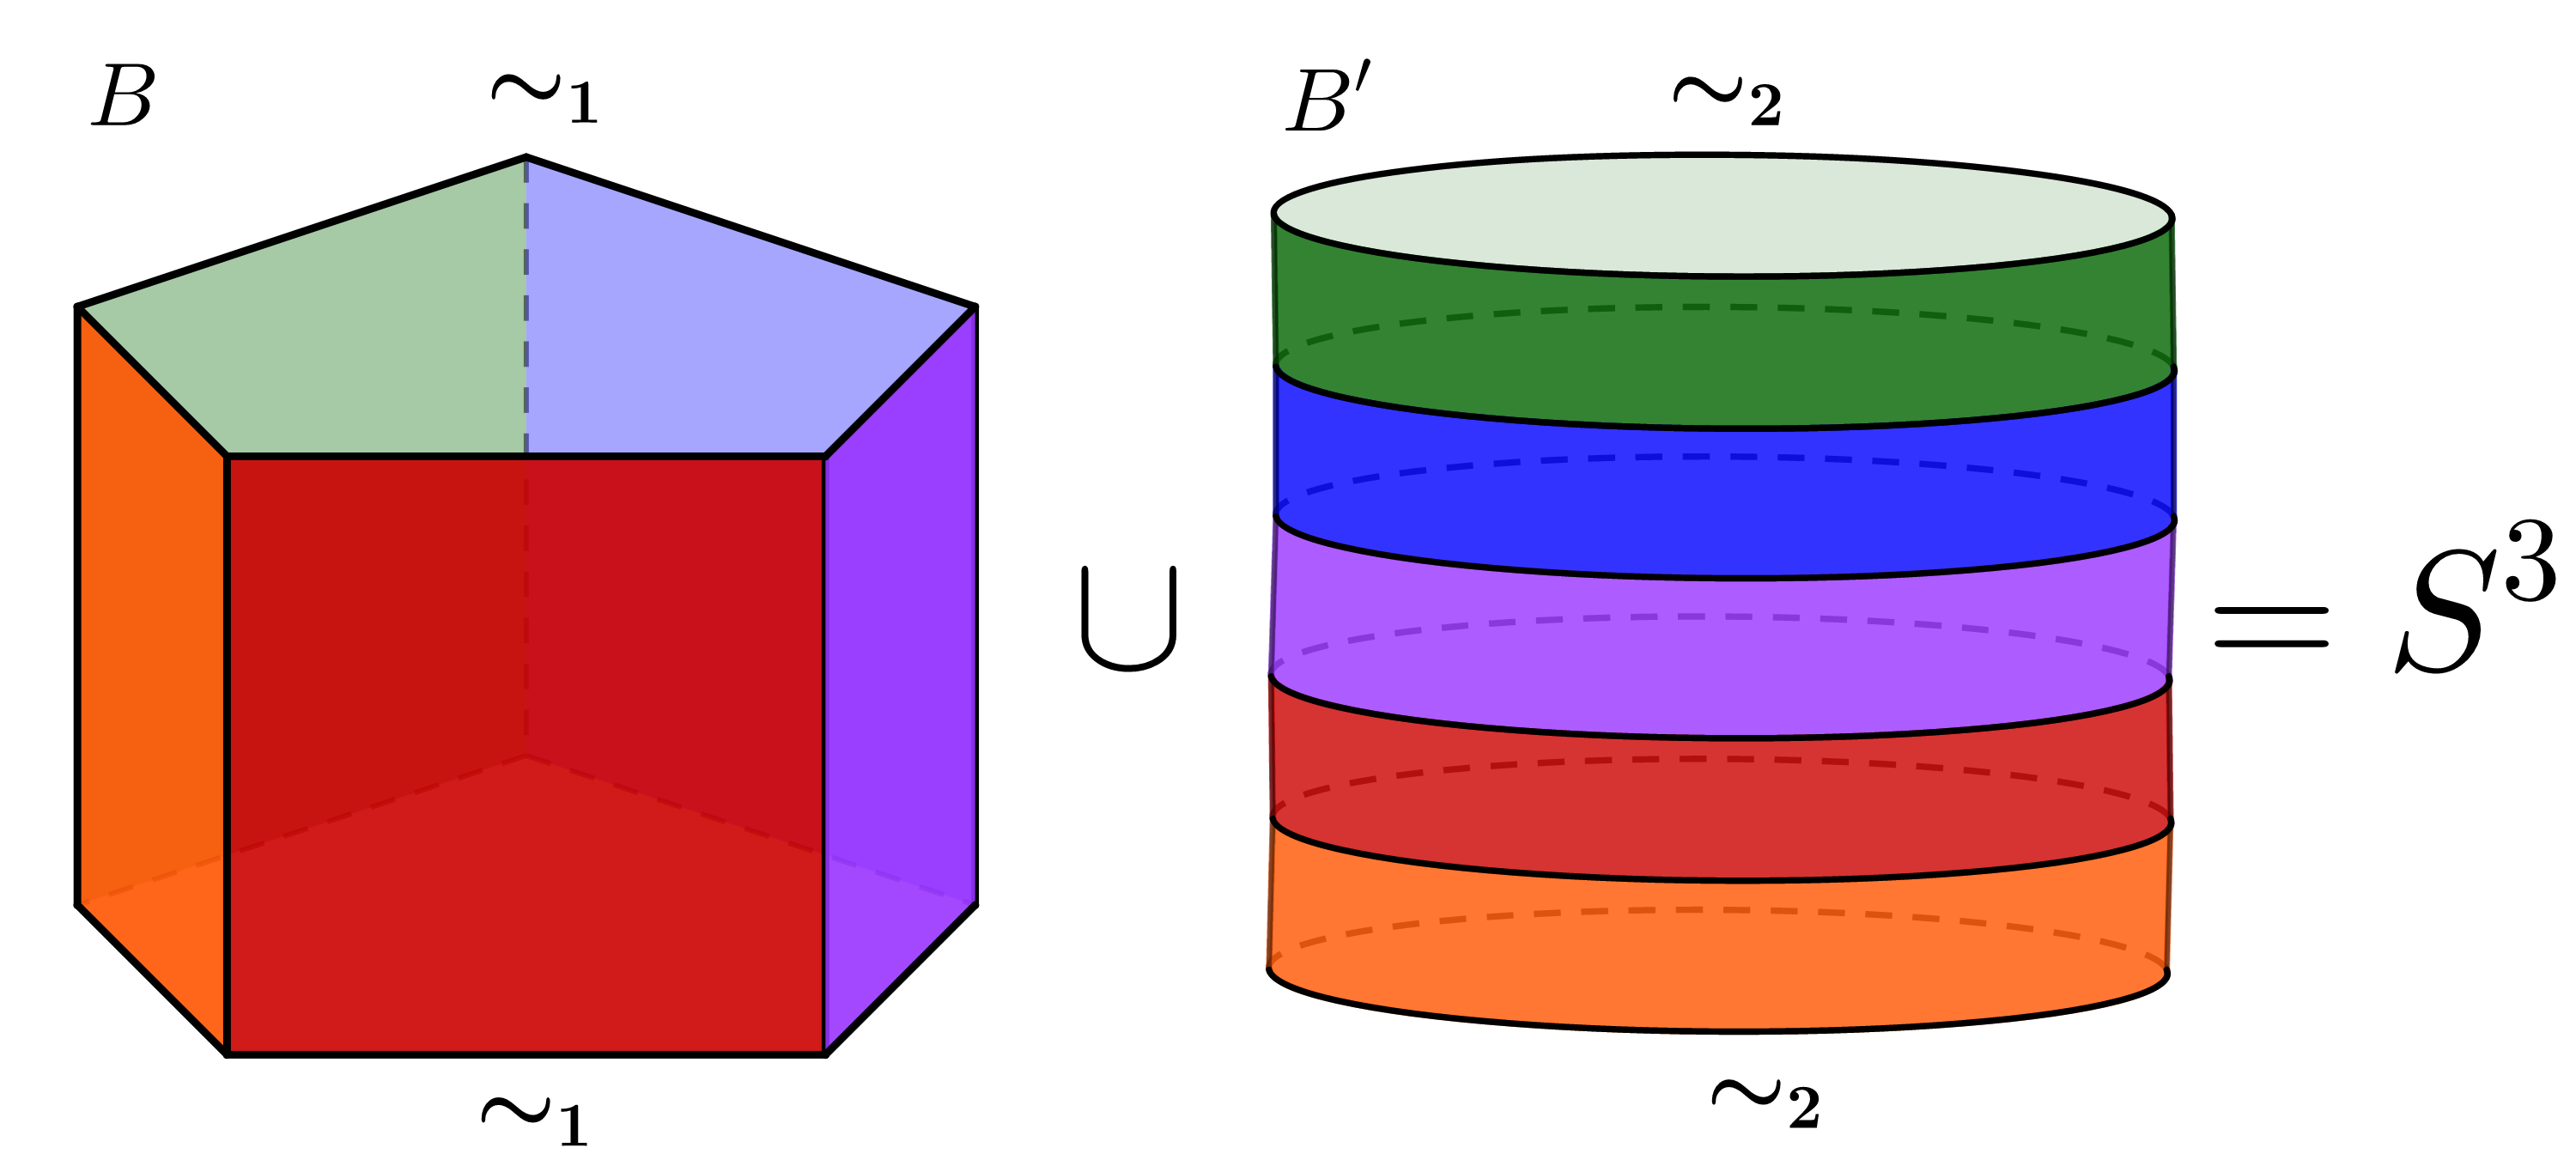
\includegraphics[width=\textwidth]{figures/face-block-complement.png}
	\caption{
		\textbf{A face block and its complement form $S^3$.}
		A face block $B$ is a stratified closed solid torus that is stratified-homeomorphic to $S^1\times G_n$ for some $n$--gon $G_n$.
		The complement of its unknotted interior in $S^3$ is another stratified closed solid torus $B'$.
		$B$ and $B'$ are depicted as cylinders with top and bottom identified.
	}
	\label{fig:face-block-complement}
\end{figure}

Taking $S_B^3$ to be the stratified $S^3$ formed as the union of $B$ and $B'$, we craft a stratified 2--handle structure as $C(S_B^3)$, the cone of $S_B^3$.
We call $C(S_B^3)$ the \emph{stratified 2--handle induced by $B$}.
Attaching $C(S_B^3)$ to $W$ over $B\subset M_1$ alters the boundary of $W$ by replacing $B\subset M_1$ with $B'$.
The full extent of this surgery can be detected by examining the edge and vertex blocks of the stratification that are incident to $B$.

\begin{theorem}
	\label{thm:primed-block-structure}
	Let $M$ be a smooth, closed, stratified, orientable 3--manifold with stratification induced by a stratifying map $f$, let $\mathfrak{B}$ be the set of face blocks of $M_1$, and let $W=M\times\Ilit$.
	Consider the 4--manifold $W'$ constructed from $W$ as
	\[
		W' = W\cup\{C(S_B^3)\}_{B\in \mathfrak{B}} / \sim,
	\]
	where $\sim$ is defined by $b\sim \iota(b)$, $\iota$ the identity map $C(S_B^3)\supset B\overset{\iota}{\to} B\subset M_1$.
	Then $M_1'=\pd W'\setminus M_0$ is a stratified 3--manifold with a decomposition into \emph{primed edge blocks} and \emph{primed vertex blocks} such that the decomposition is well-defined and the primed blocks have the following structure:
	{\renewcommand\labelitemi{}
		\begin{itemize}
			\item \textbf{Primed edge block:}
			A primed edge block $E'$ is identical to an edge block $E$ from Theorem \ref{thm:block-structure} with (3,2)--handles (i.e. cylinders: $D^2\times\Ilit$) attached over all annular boundary strata of $E$ (i.e. each closed strata $A$ of $E$ such that $A=E\cap B$ for some face block $B\in\mathfrak{B}$).
			Thus $E'$ is a stratified 3--manifold homeomorphic to $S^2\times\Ilit$
			
			\item \textbf{Primed vertex block:}
			A primed vertex block $V'$ is identical to a vertex block $V$ from Theorem \ref{thm:block-structure} with (3,2)--handles attached over each annular boundary stratum $A$ of $V$ such that $A=V\cap B$ for some face block $B\in\mathfrak{B}$.
			Furthermore, we show that $V'$ is a stratified (3,2)--handlebody.
		\end{itemize}
	}
\end{theorem}

\begin{proof}
	We split the proof of this theorem into three parts.
	In the first two parts, we prove that we can find the prescribed primed edge and vertex block structures in $M_1'$.
	In the third part, we show that these structures exhaust $M_1'$.
	
	\textbf{Part 1:}
	Edge blocks occur in three possible forms: regular edge blocks as $A\times\Ilit$, definite edge blocks as $D^2\times\Ilit$, and indefinite edge blocks as $P\times\Ilit$.
	Figure \ref{fig:edge-block-incidence} displays the possible edge block forms and indicates the boundary strata of an edge block that are shared by face blocks.
	
	\begin{figure}[h!]
		\centering
		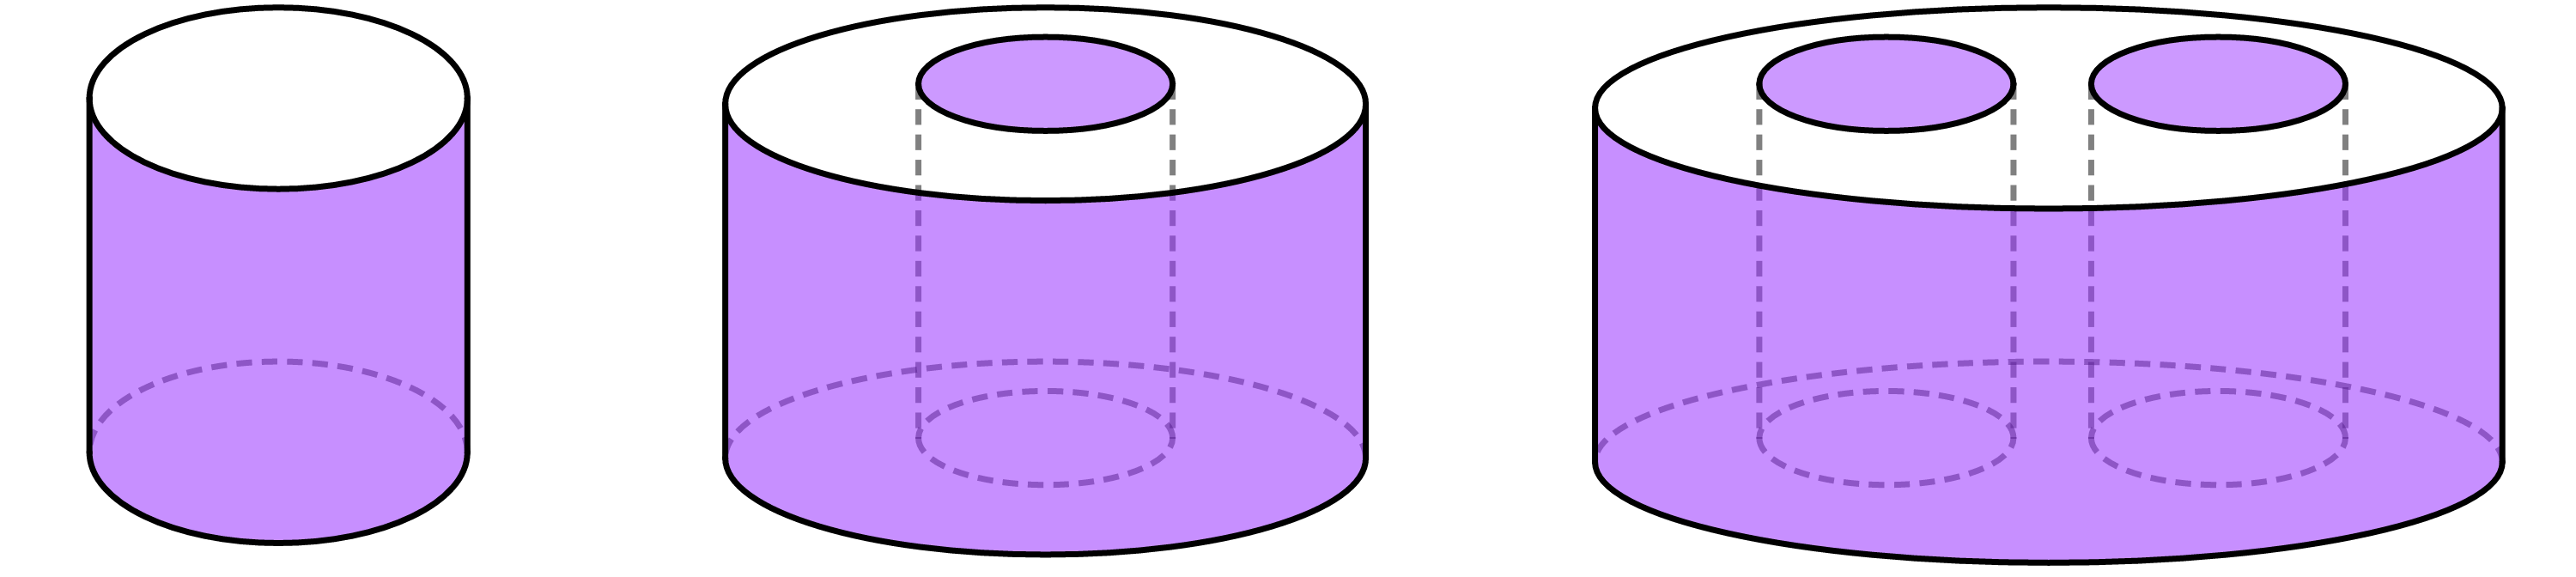
\includegraphics[width=\textwidth]{figures/edge-block-incidence.png}
		\caption{
			\textbf{Edge blocks.}
			The possible edge blocks of $M_1$.
			Annular boundary strata that are incident with face blocks of $M_1$ are indicated in purple.
			For each block, attaching (3,2)--handles over the indicated annuli results in a stratified 3--manifold homeomorphic to $S^2\times\Ilit$.
		}
		\label{fig:edge-block-incidence}
	\end{figure}
	
	Figure \ref{fig:edge-face-shared-boundary} illustrates how 2--handle attachment affects edge blocks.
%	Figure \ref{fig:edge-face-shared-boundary} shows the annulus shared by an example edge block $E$ and $B$ in $M_1$ and its corresponding annulus shared by $B$ and $B'$ in $S_B^3$.
%	The figure demonstrates that t
	The effect on $\pd W$ near $E$ of attaching the (4,2)--handle $C(S_B^3)$ over $B$ is equivalent to attaching a (3,2)--handle from the stratification of $B'$ to $E$ over the annular boundary stratum $E\cap B$.
	Attachment of all (4,2)--handles to $W$ applies this (3,2)--handle attachment to all annular strata of $E$, and attaching these (3,2)--handles to all annular strata of $E$ results in a 3--manifold homeomorphic to $S^2\times\Ilit$.

	\begin{figure}[h!]
		\centering
		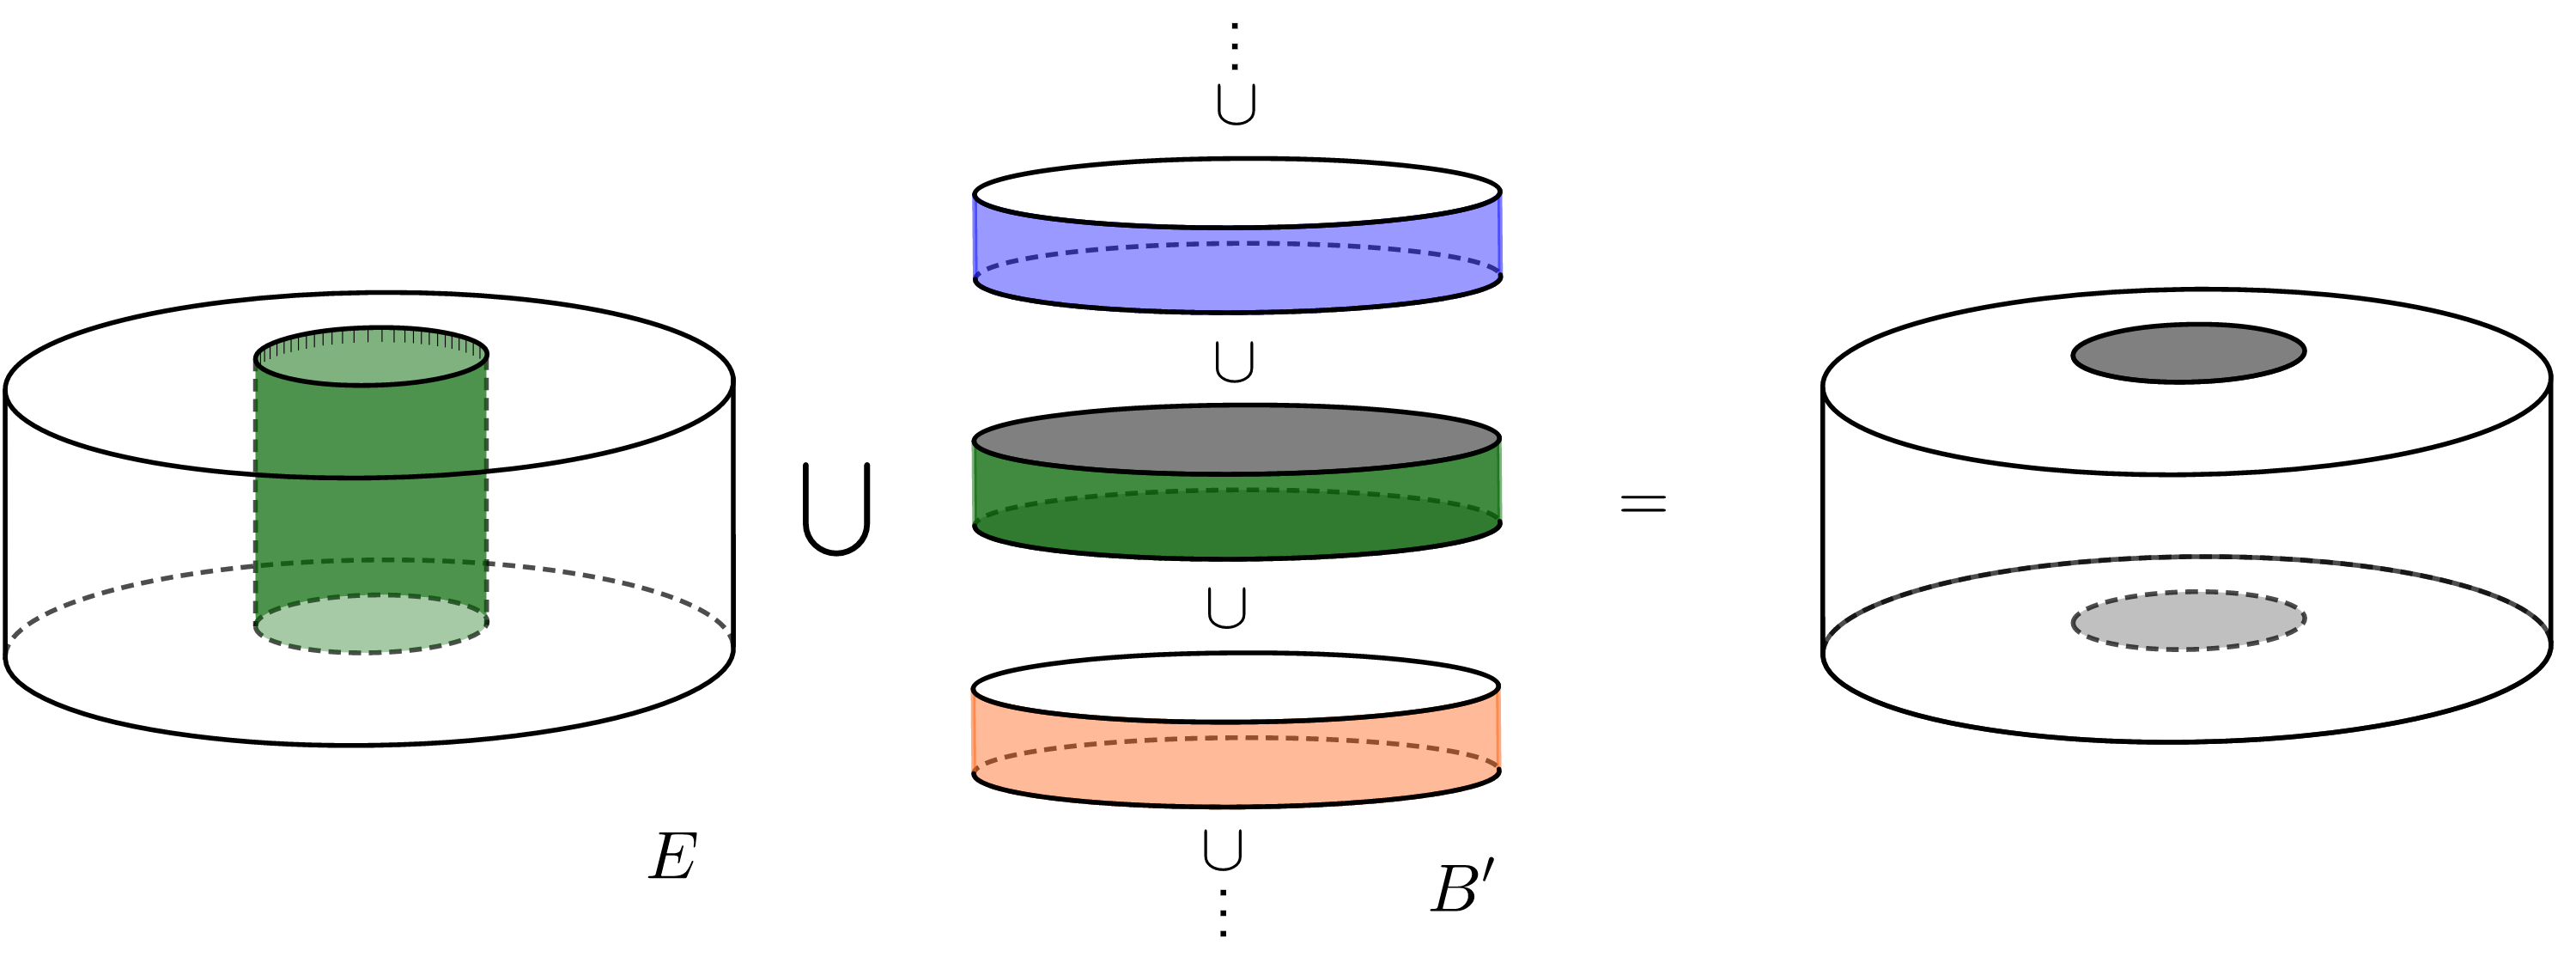
\includegraphics[width=\textwidth]{figures/edge-face-shared-boundary.png}
		\caption{
			\textbf{The effect of stratified (4,2)--handle attachment on an example edge block.}
			An edge block $E$, a face block complement $B'$, and the result of attaching $C(S_B^3)$ to $W$ over $B$ on $E$.
			The boundary stratum shared by $E$ and $B$ in $M_1$ is indicated in green, as is the corresponding boundary stratum of $B'$ in $S_B^3$.
		}
		\label{fig:edge-face-shared-boundary}
	\end{figure}
	
	\textbf{Part 2:}
	Let $V$ be a vertex block.
	All vertex blocks are stratified (3,1)--handlebodies of some genus, and
	%	The possible forms of $V$ are depicted in Figures REF.
%	Annular regions in $\pd V$ are highlighted where $\pd V$ intersects the boundary of a face block. 
%	In each case, $V$ is a (3,1)--handlebody of some genus $g$.
	$V$ and $V'$ are related via (3,2)--handle attachments to $V$ induced by (4,2)--handle attachments.
%	, and the attaching regions for these (3,2)--handle attachments are exactly the highlighted annuli in Figures REF.
	The attaching regions are disjoint, so the resulting manifold is independent of the order in which we attach handles.
	
%	\begin{figure}[h!]
%		\centering
%%		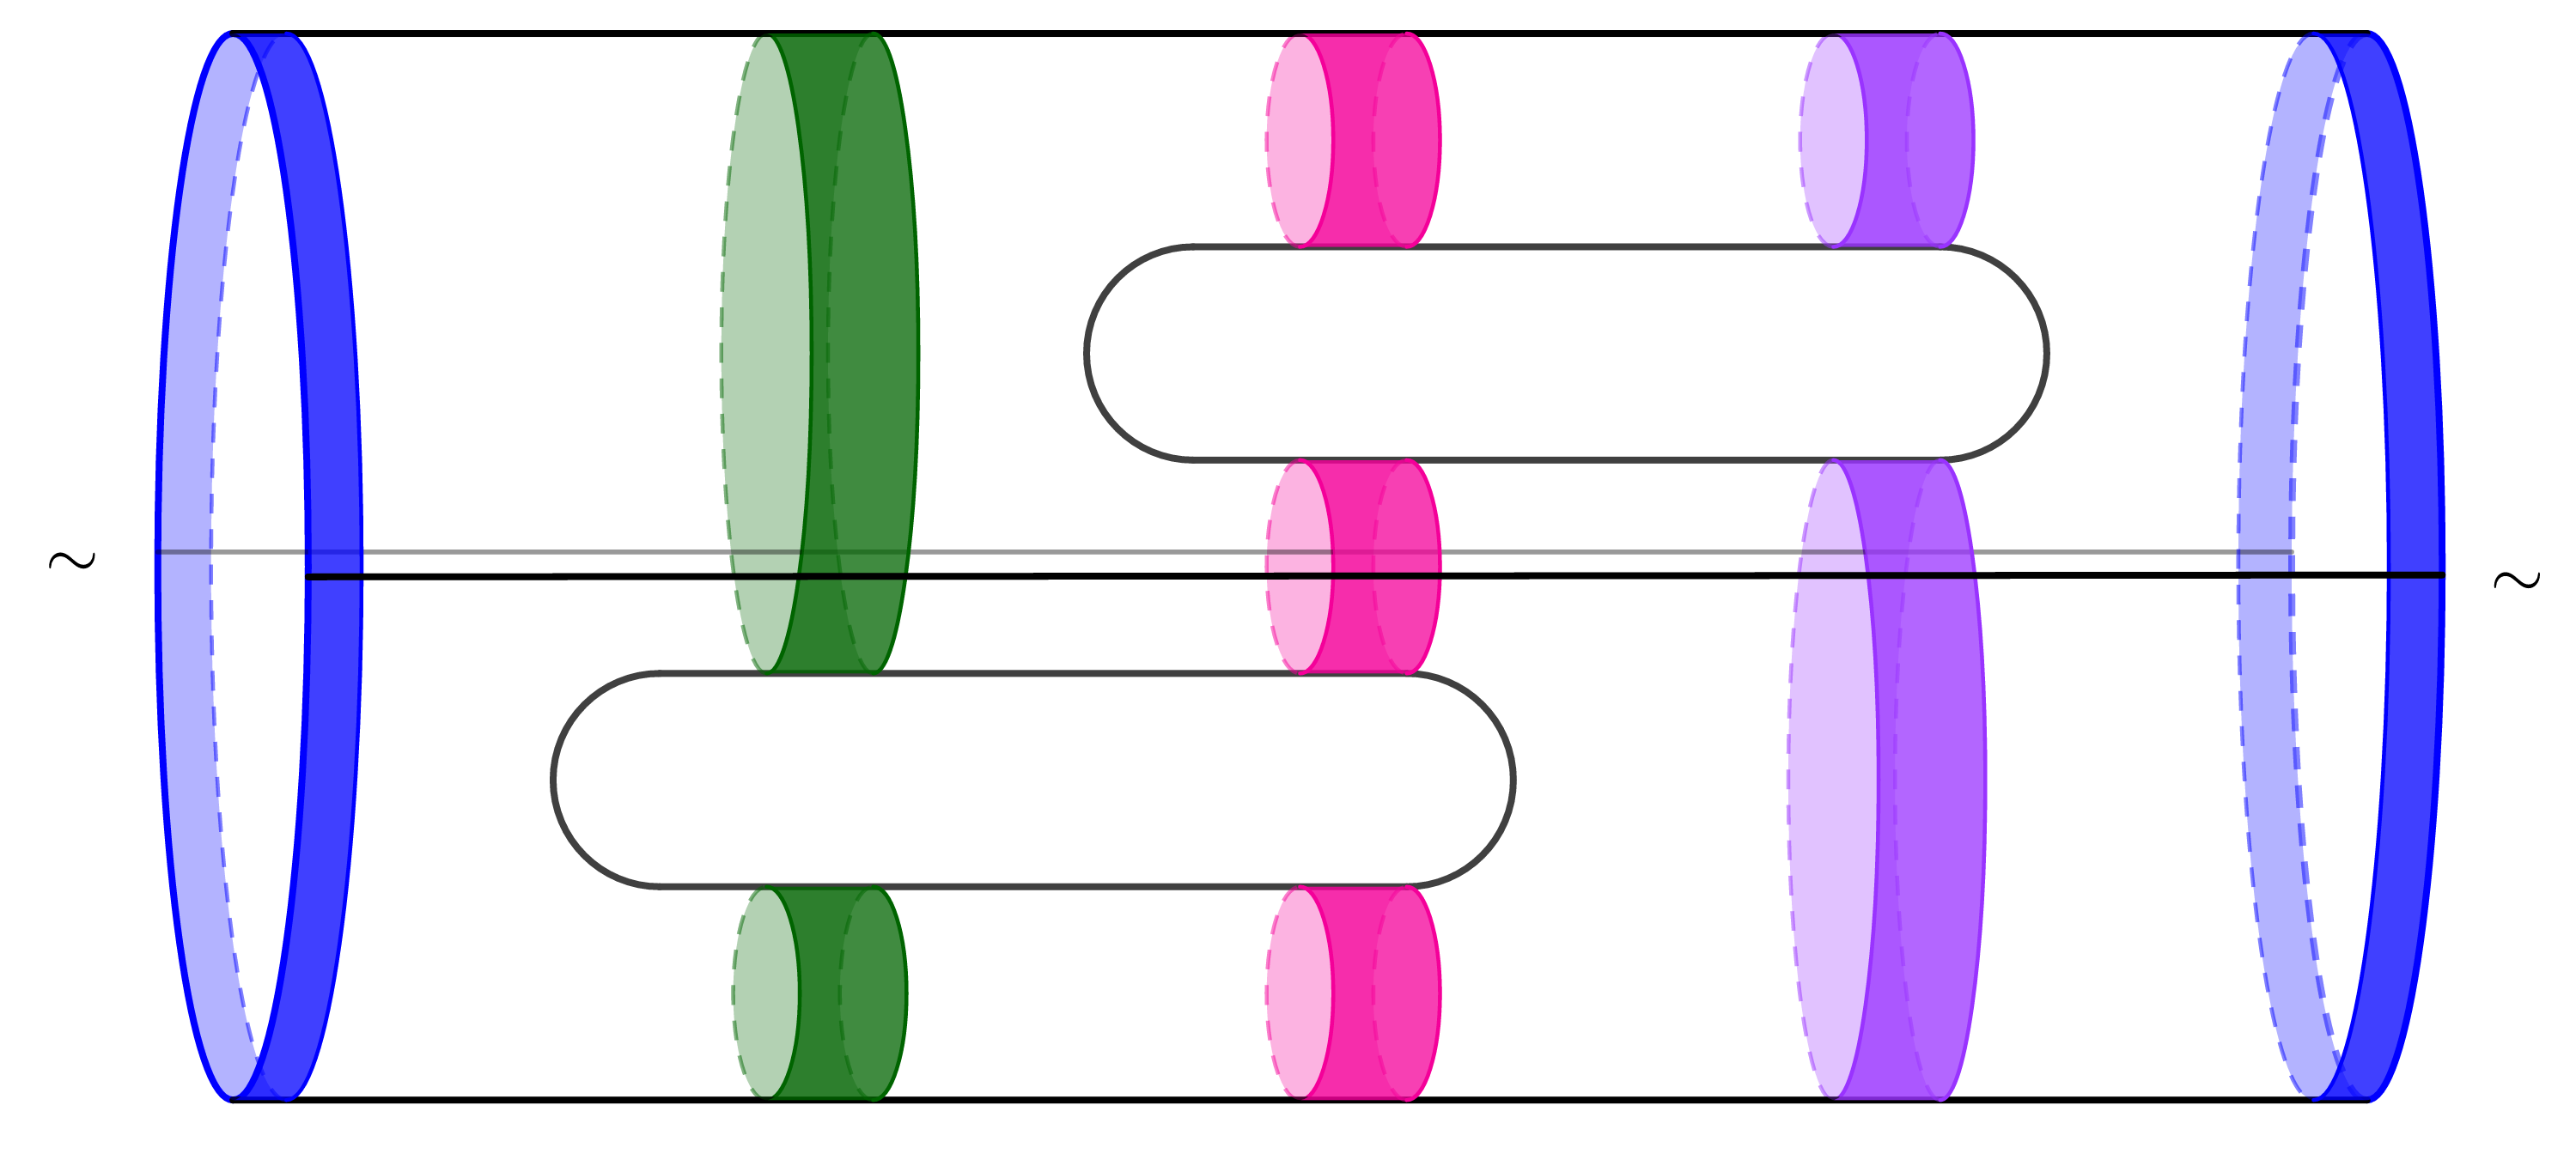
\includegraphics[width=\textwidth]{figures/vertex-block-incidence.png}
%		\caption{
%			\textbf{Vertex blocks.}
%			The possible vertex blocks of $M_1$.
%			Annular boundary strata that are incident with face blocks of $M_1$ are indicated in color and correspond to the shared vertex-face region boundary edge.
%			For each block, attaching (3,2)--handles over the indicated annuli results in a (3,2)--handlebody.
%		}
%		\label{fig:vertex-block-incidence}
%	\end{figure}
	
	Let $g$ be the genus of $V$.
	Proving that $V'$ is a (3,2)--handlebody when $g=0$ is trivial, because $V$ is then a 3--ball.
	This means $V'$ is a 3--ball with a collection of (3,2)--handles attached to it, i.e.\ a (3,2)--handlebody.
	The case of $g>0$ is nontrivial.
	
	Suppose $V$ is a (3,1)--handlebody of genus $g>0$.
	To prove that $V'$ is a (3,2)--handlebody, we show that each (3,2)--handle attachment either cancels a (3,1)--handle of $V$ or adds a new $S^2$ boundary component away from the (3,1)--handles of $V$.
	When $g>0$, $V$ is a regular neighbourhood of either a circle or one of the nontrivial singular fibers in Figure \ref{fig:saeki-fibers}.
	Each case provides a (3,1)--handlebody structure for $V$.
	Because we are interested in handle cancellation, the salient point is the identification of (3,1)--handle belt spheres.
	When $V$ is a solid torus, i.e.\ a regular vertex block, we set any meridinal circle of $V$ as a belt sphere for the (3,1)--handle.
	Otherwise, give the fiber the graph structure implied by Figure \ref{fig:saeki-fibers}.
	Then $V$ has a (3,1)--handlebody structure with one or two (3,0)--handles, depending on the number of singular points in the fiber (i.e.\ vertices in the graph structure), and a (3,1)--handle for each edge.
	
	With a (3,1)--handlebody structure in place, let $\alpha_i$ be the belt spheres of each (3,1)--handle.
	This implies that the $\alpha_i$ are pairwise non-parallel.
	Let $\beta_i$ be the attaching spheres of the (3,2)--handles that we attach to $V$ in the construction of $V'$.
	For each $i,j$, $|\alpha_i\cap\beta_j|=$ 0 or 1 by construction.
	Moreover, for every $i$, $\alpha_i\cap\{\beta_j\}_j>0$ and $\beta_i\cap\{\alpha_j\}_j>0$.
	In words, every (3,1)--handle belt sphere transversely intersects at least one of the (3,2)--handle attaching spheres, every (3,2)--handle attaching sphere intersects at least one of the (3,1)--handle belt spheres, and all intersection numbers are at most 1.
	Thus every (3,2)--handle attached to $V$ either cancels out an existing (3,1)--handle or adds a new 2--sphere boundary component.
	Because $\pd V'$ is a disjoint collection of 2--spheres we conclude that every (3,1)--handle of $V$ has been cancelled by a (3,2)--handle, thus $V'$ is a (3,2)--handlebody.
	We present an example of how these handle attachment sites are arranged in Figure \ref{fig:vertex-block-incidence}.
	
		\begin{figure}[h!]
			\centering
			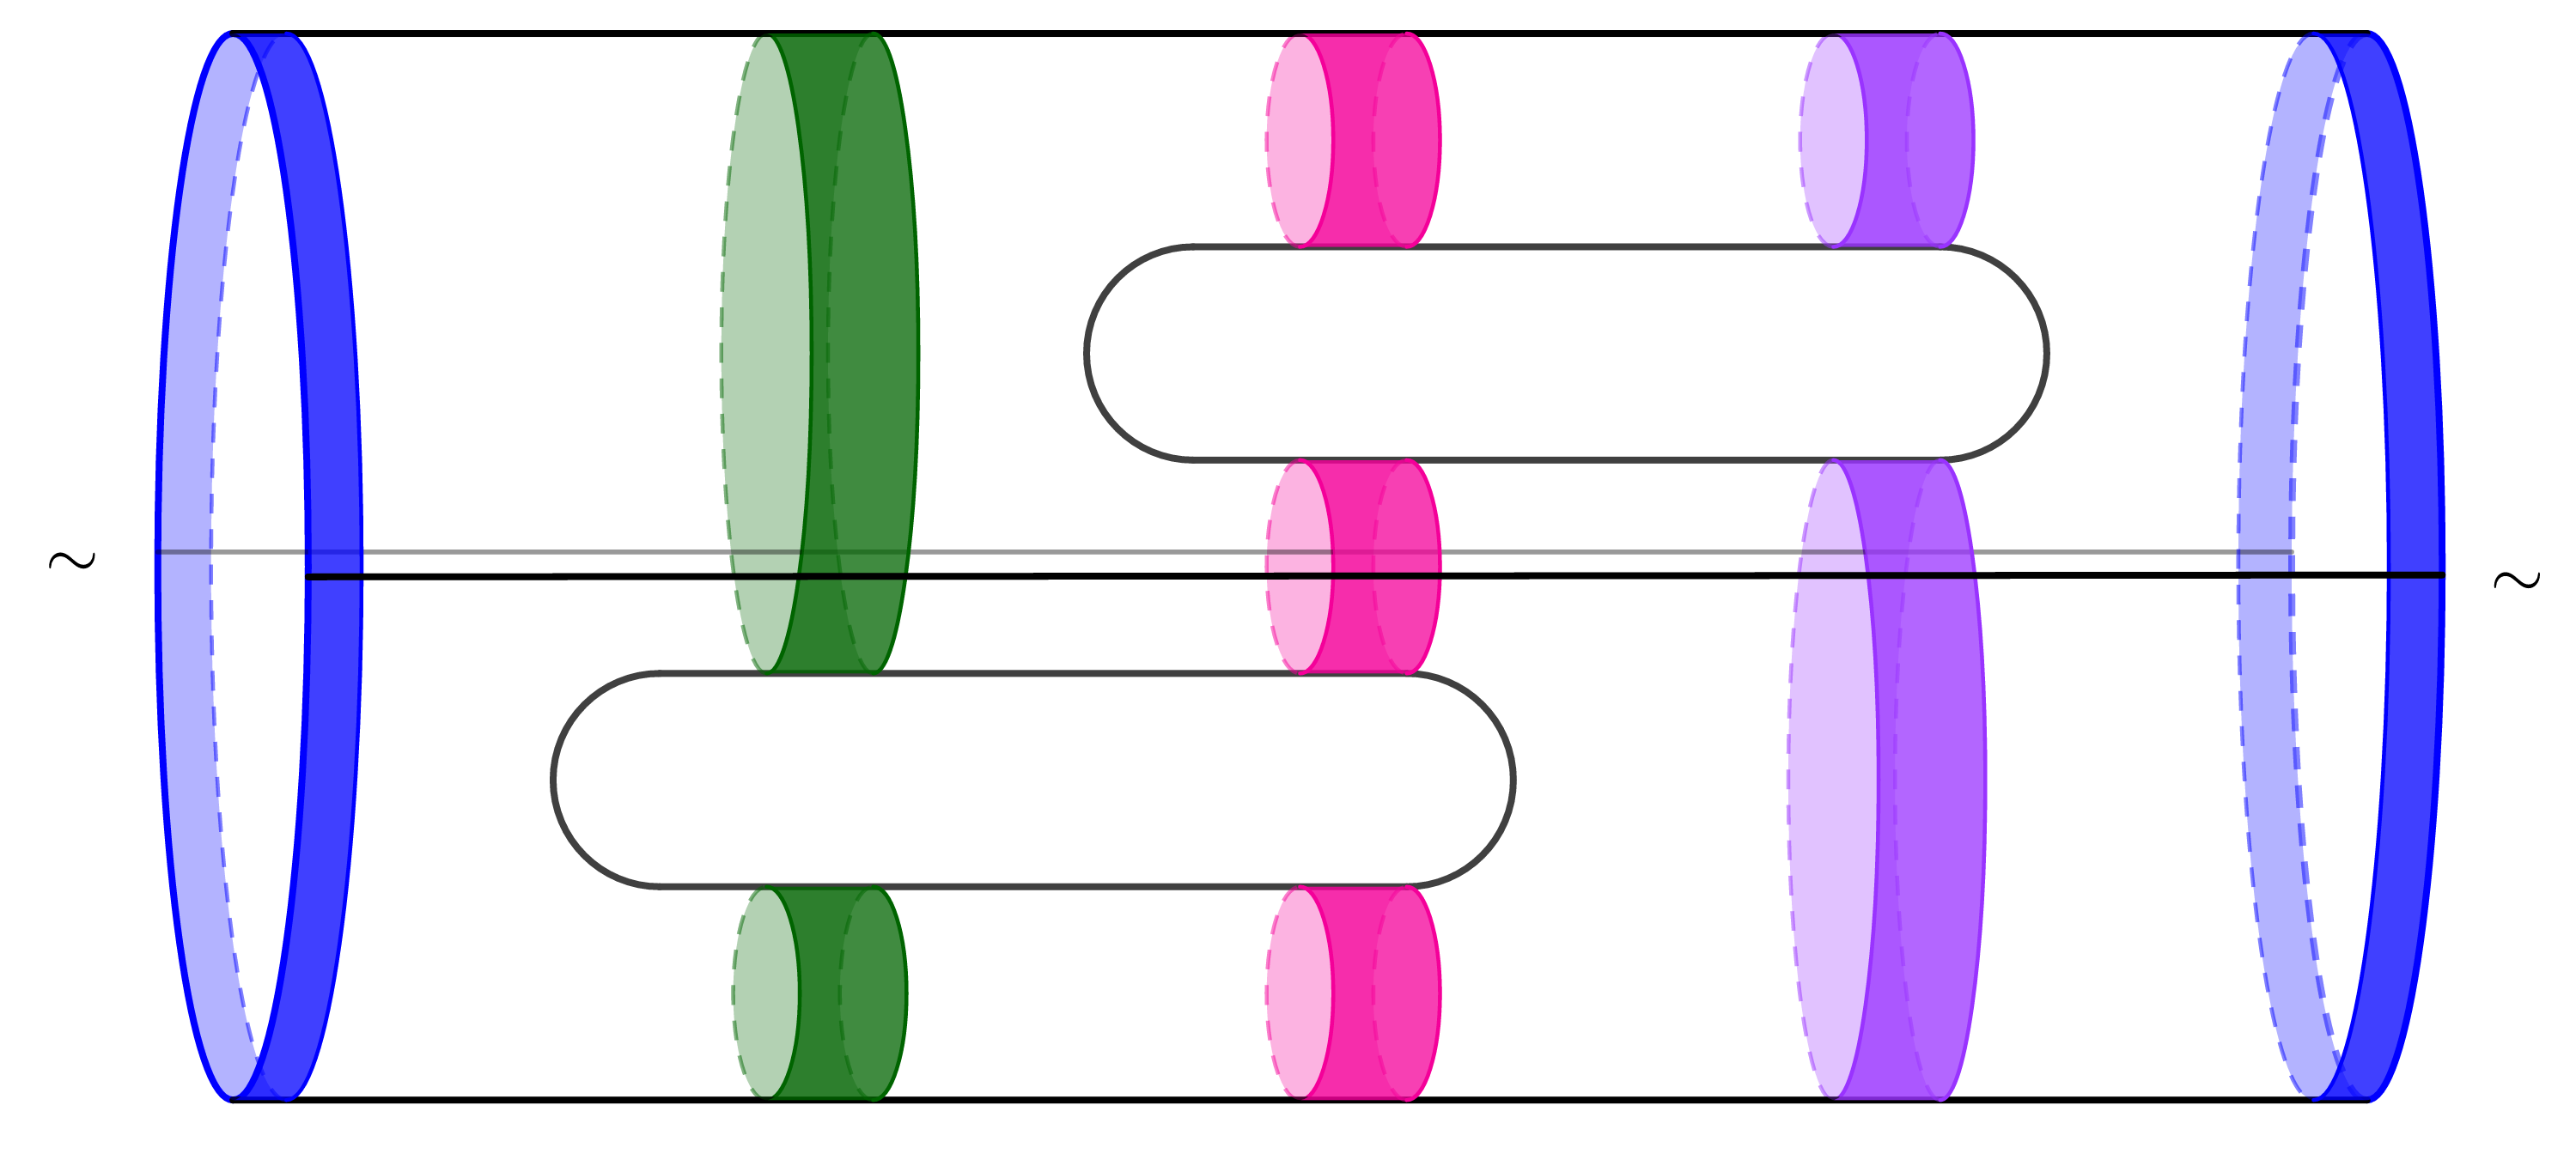
\includegraphics[width=\textwidth]{figures/vertex-block-incidence.png}
			\caption{
				\textbf{Vertex block with (3,2)--handle attachment sites indicated.}
				We display an example vertex block of $M_1$.
				Recall that this is the second type of interactive vertex block and, as in Figure \ref{fig:codim-2-surface-2}, the surface is presented as embedded in $S^3$ and the block is the stratified (3,1)--handlebody on the 'outside' of the surface in $S^3$.
				Annular boundary strata that are incident with face blocks of $M_1$ are indicated in color and correspond to the shared vertex-face region boundary edge.
				The 1--handle belt spheres are also indicated as black horizontal arcs across the surface.
				Attaching (3,2)--handles over the indicated annuli as prescribed results in a (3,2)--handlebody.
			}
			\label{fig:vertex-block-incidence}
		\end{figure}

%	Figure \ref{fig:vertex-block-incidence} displays the possible vertex block forms embedded in $S^3$ and indicates the boundary strata of a vertex block that are shared by face blocks.
%	
%	\begin{figure}[h!]
%		\caption{
%			\textbf{Vertex blocks.}
%			The possible vertex blocks of $M_1$.
%			Annular boundary strata that are incident with face blocks of $M_1$ have been indicated.
%			Gluing cylinders over the indicated annuli results in a stratified (3,2)--handlebody.
%		}
%		\label{fig:vertex-block-incidence}
%	\end{figure}	
	
%	Figure \ref{fig:vertex-face-shared-boundary} displays a model vertex block $V$ embedded on the `outside' of its stratified genus-3 boundary surface in $S^3$, and shows the annulus shared by $V$ and $B$ in $M_1$ and its corresponding annulus shared by $B$ and $B'$ in $S_B^3$.
%	The figure demonstrates that the effect on $\pd W$ near $V$ of attaching the (4,2)--handle $C(S_B^3)$ over $B$ is equivalent to attaching a (3,2)--handle from the stratification of $B'$  to $V$ over the annular boundary stratum $V\cap B$.
%	Attachment of all (4,2)--handles applies this (3,2)--handle attachment to all annular strata of $V$ shared by face blocks, and attaching these (3,2)--handles to all such annular strata of $V$ results in a 3--manifold whose boundary components are each homeomorphic to $S^2$.
%	Moreover, these boundary components are exactly the boundary components of the primed edge blocks.
	

	
%	\begin{figure}[h!]
%		\caption{
%			\textbf{The effect of stratified 2--handle attachment on a model vertex block.}
%			A model edge block $V$, a face block $B$, its complement $B'$, and the effect of attaching $C(S_B^3)$ to $W$ over $B$ on $V$.
%			The boundary stratum shared by $V$ and $B$ in $M_1$ is indicated, as is the corresponding boundary stratum of $B'$ in $S_B^3$.
%		}
%		\label{fig:vertex-face-shared-boundary}
%	\end{figure}

	\textbf{Part 3:}
	To show that primed edge and vertex blocks exhaust $M_1'$, we show that the entirety of $B'$ has been apportioned among the primed blocks for each $B'$.
	The $(3,k)$ strata of $B'$ are each cylinders whose annular boundary strata corresponds directly to a longitudinal boundary annulus of $B$.
%	Such an annulus projects through $f$ to a boundary edge of a face region.
	Face regions do not intersect even on their boundary, so all of the annular boundary strata of $B$, hence $B'$, are shared only by edge and vertex blocks.
	Thus each cylinder of $B'$ has been assigned as a (3,2)--handle and attached to a primed edge or vertex block.
	Because (4,2)--handle attachment altered $M_1$ to $M_1'$ only by replacing each face block $B$ with its complementary $B'$, the primed blocks must exhaust $M_1'$.
\end{proof}

\subsection{3--handles}
\label{subsec:smooth-3handles}

Decomposing $M_1'$ into primed edge and vertex blocks provides us with stratified 3--handle attachment neighbourhoods.
A 4--dimensional 3--handle is attached over an $S^2\times\Ilit$ embedded in the boundary of a 4--manifold, so attachment neighbourhoods for our stratified 3--handles are the primed edge blocks of $M_1'$.
We begin 3--handle attachment by precisely defining the structure of a stratified 3--handle so that it may be attached over a primed edge block.

Let $E'$ be a primed edge block of $M_1'$.
By Theorem \ref{thm:primed-block-structure}, $E'$ is homeomorphic to $S^2\times\Ilit$.
In particular, $\pd E'$ is a disjoint pair of stratified 2--spheres.
We form a 4--disk containing $E'$ in its boundary by a double coning method on $E'$: we first cone the spherical boundary components of $E'$ to form a pair of 3--disks, glue these 3--disks to $E'$ to form a 3--sphere, then cone the 3--sphere to obtain a 4--disk.

For each stratified boundary sphere $S_i^2\in\pd E'$ we form the stratified 3--disk $C(S_i^2)$ and glue $C(S_i^2)$ to $E'$ over $S_i^2$.
The result is a stratified 3--sphere, and we further cone that 3--sphere to form a stratified 4--disk.
We denote the 4--disk by $C^2(E')$ and call the resulting stratified 3--handle structure the \emph{stratified 3--handle induced by $E'$}.
Attaching $C^2(E')$ to $W'$ over $E'\subset M_1'$ alters the boundary of $W'$ by replacing $E'$ with the 3--disks $C(S_i^2)$ glued over the corresponding stratified boundary spheres in $M_1'$.
The full extent of this surgery can be detected by examining the primed vertex blocks of $M_1'$ in Corollary \ref{thm:primed-primed-block-structure}.

\begin{cor}
	\label{thm:primed-primed-block-structure}
	Let $W'$ be the 4--manifold resulting from the construction described in Theorem \ref{thm:primed-block-structure} and let $\mathfrak{E}'$ be the set of primed edge blocks of $M_1'\subset\pd W'$.
	Consider the 4--manifold $W''$ constructed from $W'$ as
	\[
	W'' = W'\cup\{C^2(E')\}_{E'\in \mathfrak{E}'} / \sim,
	\]
	where $\sim$ is defined by $e\sim \iota(e)$, $\iota$ the identity map $C^2(E')\supset E'\overset{\iota}{\to} E'\subset M_1'$.
	Then $M_1''=\pd W''\setminus M_0$ is a stratified 3--manifold with a decomposition into \emph{double primed vertex blocks} $V''$ such that the decomposition is well-defined and each $V''$ is homeomorphic to $S^3$.
\end{cor}

\begin{proof}
	We need only prove that each connected component of $M_1''$ is homeomorphic to $S^3$.
	Let $V'$ be a primed vertex block.
	We know that $V'$ is a (3,2)--handlebody and $\pd V'$ is a disjoint collection of 2--spheres.
	Thus the attachment of (3,3)--handles to $V'$ over each 2--sphere boundary component results in a 3--sphere, proving the theorem.
	
	 

%	\begin{figure}[h!]
%		\caption{
%			\textbf{Heegaard system for genus-0 vertex blocks.}
%			$V$ is a genus-0 handlebody when $V$ is a definite singular fiber of $f$.
%			There is only one possible Heegard diagram for genus-0 handlebodies, and the result is trivially $S^3$.
%		}
%		\label{fig:heegaard-genus-0}
%	\end{figure}
%
%	\begin{figure}[h!]
%		\caption{
%			\textbf{Heegaard system for genus-1 vertex blocks.}
%			$V$ is a genus-1 handlebody when $V$ is a regular fiber of $f$.
%			The Heegaard diagram consists of a meridian of each of $V$ and $H$.
%		}
%		\label{fig:heegaard-genus-1}
%	\end{figure}
%
%	\begin{figure}[h!]
%		\caption{
%			\textbf{Heegaard system for genus-2 vertex blocks.}
%			$V$ is a genus-2 handlebody when $V$ is an indefinite singular fiber of $f$.
%			The Heegaard diagram for $H$ consists of the pants cuffs, and for $V$ the side seam.
%			% we use the cuffs and the outseams from one pair of pants to form the heegaard diagram
%		}
%		\label{fig:heegaard-genus-2}
%	\end{figure}
%
%	
%	\begin{figure}[h!]
%		\caption{
%			\textbf{Heegaard system for genus-3 vertex blocks, case 1.}
%			$V$ is a genus-3 handlebody when $V$ contains an interactive singular fiber.
%			There are two types of interactive singular fibers, we show here the first from Figure \ref{fig:saeki-fibers}
%		}
%		\label{fig:heegaard-genus-3-1}
%	\end{figure}
%	
%	
%	\begin{figure}[h!]
%		\caption{
%			\textbf{Heegaard system for genus-3 vertex blocks, case 2.}
%			$V$ is a genus-3 handlebody when $V$ contains an interactive singular fiber.
%			There are two types of interactive singular fibers, we show here the second from Figure \ref{fig:saeki-fibers}
%		}
%		\label{fig:heegaard-genus-3-2}
%	\end{figure}	
\end{proof}

After attaching 3--handles over primed edge blocks, $W''$ is a 4--manifold with boundary consisting of $M_0$ and a collection of stratified 3--spheres.
We attach stratified 4--handles over these 3--spheres, so we begin by precisely defining the structure of these handles.

\subsection{4--handles}
Let $V''$ be a double primed vertex block of $M_1''$.
By Corollary \ref{thm:primed-primed-block-structure}, $V''$ is homeomorphic to $S^3$.
We form a 4--disk whose boundary is $V''$ by taking the cone of $V''$.
We denote this 4--disk by $C(V'')$ and call the resulting 4--handle structure the \emph{stratified 4--handle induced by $V''$}.
Attaching $C(V'')$ to $W''$ over $V''$ alters the boundary of $W''$ by replacing $V''$ with $\emptyset$.

\begin{cor}
	Let $W''$ be the 4--manifold resulting from the construction described in Corollary \ref{thm:primed-primed-block-structure} and let $\mathfrak{V}''$ be the set of double primed vertex blocks of $M_1''\subset\pd W''$.
	Consider the 4--manifold $W'''$ constructed from $W''$ as
	\[
	W''' = W''\cup\{C(V'')\}_{V''\in \mathfrak{V}''} / \sim,
	\]
	where $\sim$ is defined by $v\sim \iota(v)$, $\iota$ the identity map $C(V'')\supset V''\overset{\iota}{\to} V''\subset M_1''$.
	Then $M_1'''=\pd W'''\setminus M_0=\emptyset$, hence $W'''$ is a 4--manifold whose boundary is exactly $M$.
\end{cor}


